\documentclass{report}
\usepackage{standalone}

\usepackage{minted}

\newminted{python}{frame=lines}
\newminted{bash}{frame=lines}
\usepackage{tikz}
\usetikzlibrary{patterns}
\usepackage{hyperref}
\long\def\omitthis#1{\relax}

\title{ETB Guide}
\author{Sam Owre}

\begin{document}

\maketitle
\tableofcontents

\begin{abstract}

This document is a guide to the use of the \textit{Evidential Tool Bus}
(ETB).  The ETB is used to create and maintain eveidence-based arguments,
for example, for assurance cases.  The arguments are given in a variant of
Datalog, but in addition to Datalog facts, semantic attachments may be
given in the form of \emph{wrappers} to invoke external tools and create
facts.  This guide is primarily for those wanting to run the ETB and
create their own rules and wrappers.  For more on the theoretical side of
ETB, see~\cite{DBLP:conf/vmcai/CruanesHOS13,
DBLP:conf/birthday/CruanesHMOS14}.

\end{abstract}

%\section{Introduction}

\chapter{Overview}

The Evidential Tool Bus (ETB) allows different tools communicate through a
distributed \emph{tool bus}, using \emph{rules} to generate
\emph{evidence} in support of \emph{claims}.  The idea is that the rules,
evidence, and claims should provide a convincing argument to a skeptical
observer.  But beyond support for argumentation, the rules and wrappers
can form a workflow, allowing for the argument to be developed automatically, 
and rerunning the workflow as changes require, or simply to satisfy a
skeptic.

Almost any tool may be supported by the ETB, as long as a wrapper may be
written for it.\footnote{Some tools that solely support a graphic API may be
difficult, though even in this case there are usually workarounds.}  The
ETB was originally designed with formal methods tools (provers,
modelcheckers, SMT solvers, etc.) in mind, but has been extended to
include any tool.  Note that wrappers may be written that simply collect
emails, digital signatures, review notes, etc., so the notion of a tool is
fairly broad.  Wrappers are loaded when ETB starts up.

The evidence is expected to be in digital form, though this could include
pictures, digital signatures, etc., as stand-ins for physical objects.
When claims are made, e.g., that a particular file has been proved, the
file is the evidence for the claim, and it is copied into a local ETB (Git)
repository.  The actual claim then references the file by both the name
and its SHA-1 hash, which together make a \emph{file handle}.  This means
that as changes occur to files in the system, it is easily determined
which claims need to be updated.  Note the old claims are not invalid,
only valid for a different version of the file.

Rules are written in a form of Datalog.  When an ETB node starts up, it
loads the rules and wrappers, and waits for a client to issue a
\emph{query} (also known as a \emph{goal}).  Like Datalog, the answer to a
query is expected to be finite, and all the answers are returned at once.
The body (subgoals) of a matching rule is processed from left to right,
and matching variable bindings are collected.  Any subgoal that is
satisfied creates a corresponding claim, which is stored in the claims
table.  If the body is completed, the head is considered to have
succeeded, and all the corresponding instances are added to the claims
table.

The datalog term language has been extended to include JSON forms, in
particular, numbers, strings, booleans, maps (also known as objects,
records, or dictionaries), and arrays.  A file handle is actually a map,
with \texttt{file} and \texttt{sha1} fields.

ETB can run on a single machine, or it can run in a distributed framework.
The simplest runs on a local area network, ETB daemons are run on several
machines, then connected together through XML-RPC, forming a completely
connected network.  Each node has its own rules and wrappers; the
names of the predicates associated with wrappers are shared among all the
ETB nodes.  When processing a query, if it is found to match a wrapper
predicate that is handled by another ETB node, the query is sent to it,
and the answers, along with the evidence, are returned.  This is useful,
for example, when connecting tools together that run on different
platforms.

In developing a workflow for the ETB, it is best to start by deciding what
\emph{claims} you want to make to support your arguments.  In an ideal
world, all arguments are purely deductive and supported by proof.  But
real assurance cases require such issues as hazard analysis, probabilistic
arguments, test results, human factors analysis, etc.  All of these form
evidence that, e.g., a plane is \emph{safe} to fly, and it is this kind of
argument that the ETB was developed for.  See~\ref{Rushby13:safecomp} for
more discussion of these issues.

In the following we start by walking through some simple tutorial
examples, showing how to run the ETB, and how to create rules and
wrappers.  The last few chapters are a reference guide to the
language, writing wrappers, and writing ETB clients.

%\input{etb_install}
\chapter{Getting Started with ETB}
\input{etb_tutorial}
\documentclass{article}

\usepackage{tikz}
\usepackage{pgfplots}
\usetikzlibrary{patterns, backgrounds}

\title{Setting Up an ETB Network}
\author{Gr\'egoire Hamon}
\author{Ian Mason}

\long\def\omitthis#1{\relax}

\begin{document}

\maketitle

\section{Introduction}

An ETB network is composed of one or several connected ETB servers.
This network is fully connected: any server can contact any other
server directly. An ETB network can also link another ETB network
through a gateway. In this case any communication with the linked
network is done through the gateway, the linked network does not have
any knowledge of the contacting ETB network.

\section{Connected Server}

\subsection{The {\tt connect} Method}

A source ETB server can be asked to connect to a destination ETB
server using the {\tt connect} XML-RPC method:
\begin{verbatim}
connect(host, port)
\end{verbatim}
Once the connection is established, both the source and destination
propagate the information about the new server to their respective ETB
network, practically merging the two ETB networks once the propagation
is complete.

\tikzstyle{server}=[circle,draw,inner sep=0pt,minimum size=10mm, node distance=20mm]

\begin{figure}[h]
\begin{tikzpicture}[thick]
  \node[server] (A) {A} ;
  \node[server] (B) [below of=A] {B}
    edge(A);
  \node[server] (C) [right of=A] {C};
  \node[server] (D) [below of=C] {D}
    edge(C);

  \draw [->] (3.5,-1)--(5.5,-1) node [above,midway] { A.connect(C) };

 \begin{scope}[xshift=7cm]
   \node[server] (A') {A};
   \node[server] (B') [below of=A'] {B}
     edge(A');
   \node[server] (C') [right of=A'] {C}
     edge(A')
     edge(B');
   \node[server] (D') [below of=C'] {D}
     edge(A')
     edge(B')
     edge(C');
 \end{scope}
\end{tikzpicture}
\caption{Connecting Two ETB Networks}
\label{fig:connect}
\end{figure}
Figure~\ref{fig:connect} shows two ETB networks, with two servers
each, and the results of calling the {\tt connect} method of the
server {\tt A}, with the address and port of the server {\tt C}. The
resulting network contains all the servers of both networks and is
fully connected.

\subsection{Connecting a server in etb-shell}

In the etb-shell, the {\tt connect} command has exactly the same
signature as the {\tt connect} method. For example, assuming that the
etb-shell is connected to an ETB server, the command:
\begin{verbatim}
> connect(localhost, 24567)
\end{verbatim}
Calls the {\tt connect} method of the server with the arguments {\tt
  localhost} and {\tt 24567}.

\omitthis{
\section{Linked Server}

\subsection{The {\tt link} Method}

Connected servers are the normal way to establish an ETB network.
There are situation where such connection are not possible or
desirable. For example if the servers are on separate networks, it is
not always possible to get the full connectivity required by the ETB.

In such cases, ETB networks can be linked. In this mode of connection
two ETB networks communicate through a gateway server on each network.
Links have a direction: the source ETB network uses the destination
network to process queries,

An ETB server exposes a {\tt link} XML-RPC method:
\begin{verbatim}
link(host, port, my_port=NULL)
\end{verbatim}
The arguments {\tt host} and {\tt port} are the host and the port to
link to. The optional argument is used to overwrite the ETB server's
default port. It is used when communication has to go through a tunnel
-- see section~\ref{sec:using-links-connect} for details.

\begin{figure}[h]
\begin{tikzpicture}[thick]
  \node[server] (A) {A} ;
  \node[server] (B) [below of=A] {B}
    edge(A);
  \node[server] (C) [right of=A] {C};
  \node[server] (D) [below of=C] {D}
    edge(C);

  \draw [->] (3.5,-1)--(5.5,-1) node [above,midway] { A.link(C) };

 \begin{scope}[xshift=7cm]
   \node[server] (A') {A};
   \node[server] (B') [below of=A'] {B}
     edge(A');
   \node[server] (C') [right of=A'] {C}
     edge [<-,dashed] (A');
   \node[server] (D') [below of=C'] {D}
     edge(C');
 \end{scope}
\end{tikzpicture}
\caption{Connecting Two ETB Networks}
\label{fig:link}
\end{figure}
Figure~\ref{fig:link} shows the effect of linking two example ETB
networks. The server {\tt B} can use resources of the server {\tt D},
but any request is routed through the servers {\tt A} then {\tt C}.
The server {\tt C} and {\tt D} cannot use resources of either the
server {\tt A} or the server {\tt B}.

\subsection{Linking Servers Through a Tunnel}
\label{sec:using-links-connect}

When ETB servers are located on separate servers, not directly visible
from each other, they can be linked through an ssh tunnel between the
machines running the servers.

Establishing the tunnel is outside the scope of the ETB, but as an
example, let us consider the typical case of connecting two machine
separated by a firewall. We need to establish a tunnel with both local
and remote port forwarding. This is done with a command of the form:
\begin{verbatim}
ssh <user@firewall> -L <port1>:<host1>:<port2>
                    -R <port3>:<host2>:<port4> -N
\end{verbatim}
We ssh to the firewall, and establish port forwarding. The {\tt -L}
option is for the local port forwarding, {\tt port1} is the port on
which the remote ETB server is going to contact the local one, {\tt
  port2} is the actual port the local ETB server is running on.
Similarly, the {\tt -R} option is for the remote port forwarding, {\tt
  port3} is the port on which the local server is going to contact the
remote one, and {\tt port4} the port on which the ETB is running on
the remote server. When establishing a link, the optional argument to
the link method is used to pass the forwarded port instead of the
actual one.

\subsection{Establishing a Link in etb-shell}

The {\tt link} command in etb-shell is very close to the {\tt link} method:
\begin{verbatim}
> link(host, port, my_port)
\end{verbatim}
The argument {\tt my\_port} is optional, and can be used when the
linked server should contact us on port than the default ones - i.e.
if it should contact us through an ssh tunnel.

\subsubsection{Constructing a ETB SSH Tunnel Link}


We describe how to construct an ETB tunnel from a machine called {\tt etb7}
to a machine {\tt etb6} via a intermediary machine {\tt ssh1}. 
In what follows there is:

\begin{enumerate}
\item An ETB server running on {\tt  etb7} on the port 8777

\item An ETB server running on {\tt etb6} on the port 8666

\item An ssh bidirectional tunnel created on {\tt etb7} to {\tt etb6} via {\tt ssh1} using
the command:

\begin{verbatim}
etb7> ssh -L 2777:etb6:8666 -R 2666:etb7:8777  ssh.csl.sri.com
\end{verbatim}

\item An etb-shell running on  {\tt etb7} connected to the local port 8777

\end{enumerate}


To link the two servers:

\begin{verbatim}
etb7> ./etb_clients/etb-shell/etb-shell -p 8777
/ > link(localhost, 2777, 2666)
/ > 
\end{verbatim}
}


\section{Tunnels}

Connected servers are the normal way to establish an ETB network.
There are situation where such connections are not possible or
desirable. For example if the servers are on separate networks, or
one network is behind a corporate firewall, then it is
not always possible to get the full connectivity required by the ETB.

However in such cases, ETB networks can still be linked with one another, using
an {\tt ssh} tunnel.  Firstly observer that one create a two way connection
from {\tt machine1} to {\tt machine2} via a third machine 
{\tt firewall}, by executing the two ssh commands:

Firstly, on  {\tt machine2} 

{\small
\begin{verbatim}
ssh -v -L "Proxy port A":"machine1":"Port A" -R "proxy":"machine2":"Port B"  "firewall" -N
\end{verbatim}
}

and, secondly on {\tt machine1}

{\small
\begin{verbatim}
ssh -v -L "Proxy port B":"firewall":"proxy"  "firewall" -N
\end{verbatim}
}

the situation that results is indicated in the picture \ref{fig:sshtunnel}

\begin{figure}
\begin{center}
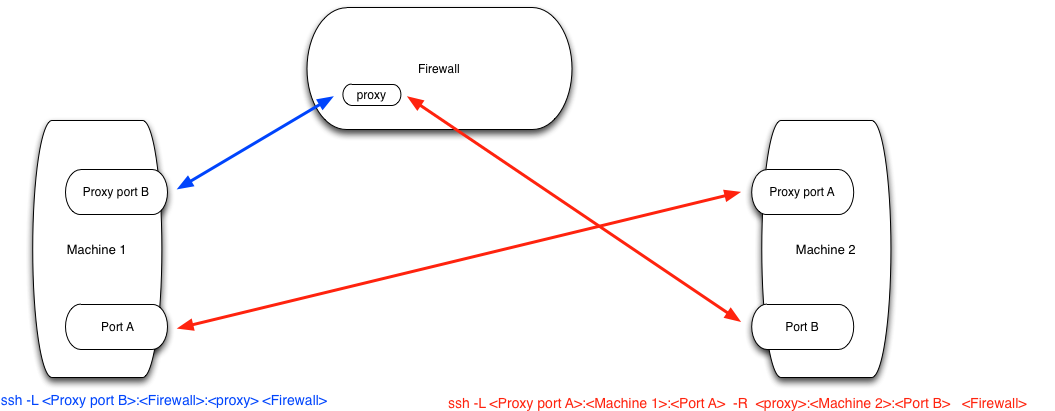
\includegraphics[scale=.30]{images/sshTunnel}
\caption{Ssh Tunnel Scenario}\label{fig:sshtunnel}
\end{center}
\end{figure}

Assuming that we have ETB servers running on these two connected machines
we can connect them by either the 
\begin{verbatim}
etb shell on machine2> tunnel("Proxy port A", "Proxy port B")
\end{verbatim}
or symmetrically 
\begin{verbatim}
etb shell on machine1> tunnel("Proxy port B", "Proxy port A")
\end{verbatim}

the situtaion that results in either case is indicated in the picture \ref{fig:2waytunnel}

\begin{figure}
\begin{center}
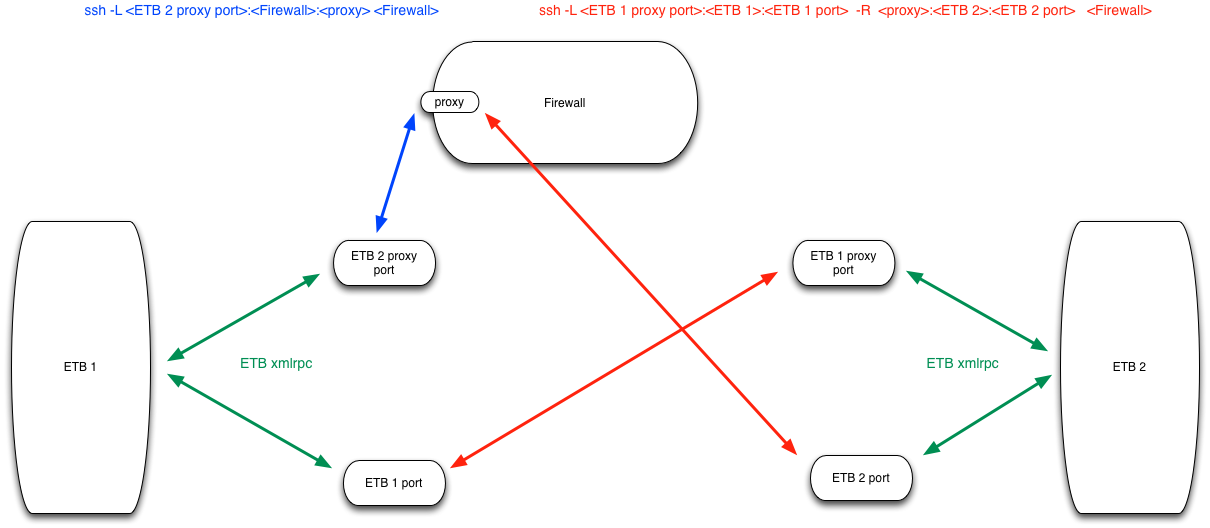
\includegraphics[scale=.30]{images/2waytunnel}
\caption{The Two Way Tunnel Scenario}\label{fig:2waytunnel}
\end{center}
\end{figure}

\subsection{The {\tt tunnel} Method}


An ETB server exposes a {\tt link} XML-RPC method:
\begin{verbatim}
tunnel(localport, remoteport)
\end{verbatim}
The arguments {\tt localport} and {\tt remoteport} correspond to 
the local proxy port on the network executing the  {\tt tunnel}
command, and the remote proxy port on the remote network.


\subsection{A {\tt tunnel} Use Case}

In order to make things more concrete, lets give a detailed 
example of doing a distributed make on two ETB networks
separated by a firewall, but connected by a tunnel.

In particular we will link a network running on a Macbook pro
{\tt pepper} with a Linux server {\tt iandev} running in SRI's cloud. 
The Macbook pro will be behind the CSL's firewall {\tt thor.csl.sri.com}.


So to begin with we start ETB servers on both machines, to make thing easier to
keep clear in our head, ports with {\tt 6}s in them will be on the Macbook,
while ports with {\tt 7}s in them will be on the Linux server. The sole
port on {\tt thor.csl.sri.com} that enters the fray will have {\tt 5}s in it.

The {\tt start} script in the {\tt demos/make} directory will accept
a port argument and start an ETB server running on that port, (and if the port is specified, 
the server will start in debug mode), otherwise it will use the default port specified
in the {\tt etb\_conf.ini} file.
\begin{verbatim}
pepper>cd etb/dmoes/make
pepper>./start 8666
...
\end{verbatim}
and 
\begin{verbatim}
iandev>cd etb/demos/make
iandev>./start 8777
...
\end{verbatim}
Now in order to connect these two networks, we first need to setup a two way {\tt ssh}
tunnel, firstly on {\tt iandev}:

\begin{verbatim}
ssh -v -L 2777:pepper:8666 -R 2555:iandev:8777  thor.csl.sri.com -N
\end{verbatim}
and secondly on {\tt pepper}:

\begin{verbatim}
ssh -v -L 2666:thor.csl.sri.com:2555  thor.csl.sri.com -N
\end{verbatim}

At this point we can test our connectivity simply using python's
command line, for example on pepper we could do:

\begin{verbatim}
import xmlrpclib
server = xmlrpclib.Server("http://localhost:2666")
server.system.listMethods()
server.get_id()
\end{verbatim}

which should return the id of the server running on {\tt iandev}, similarly 
we could do the reverse on {\tt iandev}, simply by using the 
URI {\tt "http://localhost:2777"}.

Now assuming that the above went smoothly, we can run an {\tt etb-shell}
on {\tt pepper}, and connect the two networks:
\begin{verbatim}
pepper>cd etb/demos/make
pepper>../../etb_clients/etb-shell/etb-shell -p 8666
/ > tunnel(2666, 2777)
\end{verbatim}
we could now do a compile on {\tt iandev} by doing:
\begin{verbatim}
# We first put all of our files on pepper
h1 = put_file(component1.h)
src1 = put_file(component1.c)
h2 = put_file(component2.h)
src2 = put_file(component2.c)
srcMain = put_file(main.c)
# Build everything, wait, then get the exe back
q = main("Linux_x86_64", src1, h1, src2, h2, srcMain, "main_Linux_x86_64", Exe)
r = query_wait(q)
get_file(r.Exe, "main_Linux_x86_64")
\end{verbatim}
once this has finished successfully we could do a similar feat on {\tt iandev}:
\begin{verbatim}
iandev>cd etb/demos/make
iandev>../../etb_clients/etb-shell/etb-shell -p 8777
\end{verbatim}
Note that it is not necessary to do the tunnel on this side, since the effect is
symmetric. Before we try and compile on the remote Macbook, first observe
that while the necessary files have been copied over to the linux server,
we have no way of referring to them, and thus no way to ask for the compilation to take place.

So to begin with we ask for handles to the existing files in the servers git repository,
using the the {\tt get\_filehandle} command:
\begin{verbatim}
h1 = get_filehandle(component1.h)
src1 = get_filehandle(component1.c)
h2 = get_filehandle(component2.h)
src2 = get_filehandle(component2.c)
srcMain = get_filehandle(main.c)
\end{verbatim}
We can now ask the appropriate query:
\begin{verbatim}
q = main("Darwin_i386", src1, h1, src2, h2, srcMain, "main_Darwin_i386", Exe)
\end{verbatim}




\end{document}

%\input{etbd}
%\input{etbsh}
%\input{etb_language}
\chapter{ETB Wrappers}
\documentclass{article}

\usepackage{minted}

\newminted{python}{frame=lines}

\title{ETB Wrappers}
\author{Gr\'egoire Hamon, Ian A. Mason}

\begin{document}

\maketitle

This document describes the integration of a tool with the {\it
  Evidential Tool Bus} (ETB). This integration consists in writing a
wrapper for the tool, the wrapper exposes the tool to the ETB in the
form of predicates.

\section{Introduction}

A tool wrapper for the ETB is a Python class. Some methods of the
class are declared as {\it predicates} and are seen as such by the
ETB. Predicates can be implemented directly in Python or make calls to
external tools or libraries. Being regular Python classes, wrappers
can contain any code beside predicates.

The ETB provides support to write tools wrapper in the form of a
Python library. This document describes the use of this library. We
consider external command-line tools as examples, but the same
principles apply to libraries.

\section{Tools and Predicates}

A tool is something that the ETB can call to establish or verify a
claim. It can be an external command-line tool, a library, or a Python
function. 

A tool wrapper is a collection of predicates. Predicates from the
Python point of view, are methods of the wrapper class that have a
predicate specification.

\subsection{The {\tt Tool} Class}

A tool wrapper should inherit from the {\tt Tool} class. This class
defines a decorator for predicate specification, as well as generic
utility functions to get the predicates associated with a tool, get
the signature of a predicate, or report an error within the tool to
the ETB. Higher level classes are also available, for example {\tt
  BatchTool} or {\tt InteractiveTool}.

\subsection{Predicate Specification}

A predicate is a method of the wrapper class that is decorated using
{\tt Tool.predicate}. The {\tt Tool.predicate} decorator takes as
argument a string representation of the predicate's signature.

The signature is a comma separated list of arguments to the
predicate. Each argument is of the form {\tt <sign><name>: <kind>}
where {\tt <sign>} is either {\tt +} or {\tt -} and indicates whether
the argument is read or written, {\tt <name>} is a variable name, and
{\tt <kind>} is the kind of this variable and can be either {\tt
  value}, {\tt file} or {\tt handle}. For example, the signature of a
predicate {\tt bmc} that checks if a property {\tt P} is valid for a
model {\tt M} up to depth {n} could be:
\begin{pythoncode}
@Tool.predicate('+property: value, +model: file, +depth: value,
                 -valid: value')
\end{pythoncode}
Note that the specification only indicates the kind of the predicates
arguments, not their type. This is used to make sure that files are
synchronized between ETB nodes, or that handles are consistent. Values
are not interpreted or validated by the ETB, this is left to the tool.

\section{Batch Tools}

Batch tools are the easiest to plug into the ETB. These are tools for
which each predicate can be invoked in isolation.

\subsection{The {\tt BatchTool} Class}

The {\tt BatchTool} class in the module {\tt structs} can be used to
write a wrapper for a batch tool. The class offers infrastructure to
call a tool as an external process or parse the results coming from
that external process. The main method is {\tt run}:
\begin{pythoncode}
  wrapper.run(result, *args)
\end{pythoncode}
calls the command specified by {\tt *args}, parses the output and
returns it in {\tt result}. Intermediate methods are called to call
the tool ({\tt callTool}) parse ({\tt parseResult}) or interpret ({\tt
  bindResult}) the output and can be overriden as needed.

\subsection{Example: A {\tt SAL} Batch Wrapper}

We would like to write a wrapper for the SAL tool suite. The suite is
composed of a set of batch tools with very similar interfaces: most
tools are called with a set of flags, the name of a SAL context, which
is also the name of a sal file, and often the name of a property.

We start a new class, {\tt SalBatch}, which is a {\tt BatchTool}:
\begin{pythoncode}
class SalBatch(BatchTool):
  """Batch wrapper for SAL"""
\end{pythoncode}

We first define a predicate to call the SAL symbolic model-checker,
{\tt sal-smc}. Our predicate has the following signature:
\begin{pythoncode}
  @Tool.predicate("+Model:file, +Prop:value, -Result:value")
\end{pythoncode}
The predicates states that analyzing the property {\tt prop} for {\tt
  model} gives {\tt result}. {\tt model} is the name of a SAL file,
{\tt prop} is the name of the property to be analyzed, and {\tt
  result} is a variable. 

We can now write the code for the predicate:
\begin{pythoncode}
  def sal_smc(self, model, prop, result):
    sal_smc = 'sal-smc'
    (context, _) = os.path.splitext(model)
    return self.run(result, sal_smc, context, prop)
\end{pythoncode}
We first define the command that we want to call, and prepare its
arguments: The command is simply the string {\tt 'sal-smc'}, we
extract the name of the context from the file name by removing its
extension. Finally, we can call the method {\tt run}, and return its
result: it first invoke the command with the arguments {\tt context}
and {\tt prop}. It then parses its output and binds the result to {\tt
  result}. This process invokes three methods of the class {\tt
  BatchTool} that can be redefined as needed: {\tt callTool} call the
commands and returns its standard output as a string, {\tt
  parseResult} takes that string and produces the result in the
desired format, and {\tt bindResult} binds it to the result
variable. In this example, we use the default implementation of these
methods.

Very similarly, we can add a predicate to check for deadlocks:
\begin{pythoncode}
@Tool.predicate("+model:file, +module:value, -result:value")
def sal_deadlock_check(self, model, module, result) :
  ctx = self.context_from_filename(model)
  return self.run(result, 'sal-deadlock-checker', ctx, module)
\end{pythoncode}
This is exactly as before, we factorized the extraction of the context
name in a method {\tt context\_from\_filename}. Following this model,
we can wrap all the SAL batch commands.

\section{Returning Results from Tools}

In addition to the  {\tt Tool} class is the {\tt Result} class hierarchy,
which is designed to encapsulate the values returned from external tools.

The most common way of returning information to the ETB is by way of a 
substitution, or binding, of values to variables. A substitution is
simply a list of bindings, obtained using  {\tt bindResult}, and returned
to the ETB using the {\tt Substitutions} class.

\begin{pythoncode}
    @Tool.predicate('+a: value, +b: value, -res: value')
    def plus(self, a, b, res):
        a = a.get_val()
        b = b.get_val()
        if res.is_var():
            return Substitutions(self, [self.bindResult(res, a+b)])
        else:
            res = res.get_val()
            return Success(self) if res == a + b else Failure(self)
\end{pythoncode}

The first argument to the {\tt Substitutions} constructor is the tool itself,
the second is a list of substitutions. The interpretation being that 
each substitution satisfies the goal represented by the tool wrapper call.

{\tt Success} and {\tt Failure} are simply convenient abbreviations
for 

\begin{pythoncode}
Substitutions(self, [{}])
Substitutions(self, [])
\end{pythoncode}
respectively.


An example of returning a non-trivial list of substitutions is given
by the {\tt in\_range} example, that for each element in the
range  {\tt [low, up]} returns a substitution binding {\tt res}
to that element.

\begin{pythoncode}
    @Tool.predicate("+low: value, +up: value, -res: value")
    def in_range(self, low, up, res):
        """Result in [low, up] range."""
        low = int(low.val)
        up = int(up.val)
        if low > up:
            return Failure(self)
        if res.is_var():
            slist =  [self.bindResult(res, i) for i in range(low, up+1)]
            return Substitutions(self, slist)
        else:
            res = int(res.val)
            if low <= res <= up:
                return Success(self)
            else:
                return Failure(self)
\end{pythoncode}





\section{Interactive Tools}

Interactive tools require more machinery as the ETB needs to keep a
session open with the tool, and needs to keep track of what is
happening in a given session so that a claim can be replayed.

The communication between the ETB and the tool is also more involved,
as the ETB needs to know when a tools is communicating with it.

\subsection{The {\tt InteractiveTool} Class}

The {\tt InteractiveTool} class can be used as a starting point to
wrap interactive tools. It offers methods to:
\begin{itemize}
\item connect to a tool running as an external command {\tt connect}
\item communicate with this tools through {\tt stdin} ({\tt write} and
  {\tt stdout} ({\tt read})
\item takes care of managing sessions {\tt updateSession}
\end{itemize}
The default implementation makes assumptions about the protocol used
to communicate with the tool, but as for the batch case, these
assumption are encoded within methods that can be overridden:
\begin{itemize}
\item every message send to the tool is followed by a response
\item the response is read line by line
\item a response is complete if the method {\tt parse\_stop} applied
  to the last line read returns true (by default the empty string)
\item the method {\tt parse\_error} takes a response and raise an
  exception is the response contains an error message. It returns {\tt
    None} otherwise (default: always return {\tt None})
\item the method {\tt parse\_output} transform the response in a form
  suitable for the ETB (default: identity)
\end{itemize}

\subsection{Example: {\tt sal-sim}}

As a running example, we are going to write a wrapper for the SAL
simulator. The simulator is started through the command {\tt sal-sim},
then lets the user step through simulations of a model through a
read-eval loop. The wrapper is an {\tt InteractiveTool}:
\begin{pythoncode}
class SALsim(InteractiveTool):
  """ETB wrapper around SALsim."""
\end{pythoncode}
The first thing to do is to start the tool, and get a handle to
communicate with it. For {\tt sal-sim}, we define the following
method, which calls the command, then import the model we want to
simulate, starts the simulation and returns a handle to the ETB:
\begin{pythoncode}
  @Tool.predicate("+Model: file, +Module: value, -Session: handle")
  def salsim_start(self, model, module, session) :
    (ctx, ext) = os.path.splitext(model)
    s = self.connect('sal-sim')
    self.write(s, '(import! "%s")\n' % ctx)
    self.write(s, '(start-simulation! "%s")\n' % module)
    return  Substitutions(self, [ self.bindResult(session, s) ])
\end{pythoncode}
The {\tt connect} method of {\tt InteractiveTool} call the command,
registers the session and gives us a handle to the session back. Using
this handle, we can call the method {\tt write} to send commands to
the tool.

The next predicates lets us get the current states of the system, by
calling the simulator command {\tt (display-curr-states)}:
\begin{pythoncode}
    @Tool.predicate("+Session: handle, -States: value")
    def salsim_current_states(self, session, states) :
        out = self.write(session, '(display-curr-states)\n')
        return  Substitutions(self, [ self.bindResult(states, out) ])
\end{pythoncode}
We send the command to {\tt sal-sim} and return the output as-is. Note
that the output of that command is a textual representation of the
states, and would probably need to be parsed, which we are not doing
here.

We now move on to a more complex predicate, which is changing the
session:
\begin{pythoncode}
    @Tool.predicate("+SessionIn: handle, -SessionOut: handle")
    def salsim_step(self, sessionIn, sessionOut) :
        self.write(sessionIn, '(step!)\n')
        slist = [ self.bindResult(sessionOut, self.updateSession(sessionIn)) ]
        return Substitutions(self, slist)
\end{pythoncode}
{\tt salsim\_step} causes the running simulation to take a step. The
predicates takes the session to advance as argument and returns a new
session. The input session becomes unavailable. This is implemented by
calling the command, then using the {\tt updateSession} method.

Finally, we can have a predicate to close the session:
\begin{pythoncode}
    @Tool.predicate("+Session: handle")
    def salsim_close_session(self, session) :
        self.write(session, '(exit)\n')
        return Failure(self)
\end{pythoncode}

\section{Registering Tools and Rules}

\subsection{Registering a Tool}

Once a wrapper class has been written for a tool, it still needs to be
instantiated and registered with the ETB. A wrapper should be in a
Python file that contains a {\tt register} function. This function is
executed by the ETB when the file is loaded. As an example, to
register the {\tt SalBatch} wrapper, we write:
\begin{pythoncode}
def register(etb):
  "Register the tool"
  etb.add_tool(SalBatch(etb))
\end{pythoncode}


\subsection{Generating Queries}

As a prequel to describing the ability to add rules dynamically,
we illustrate the ability to generate and add simple queries
to the ETB system.
In this example we have two mutually {\em recursive} predicates
{\tt ping(M)} and {\tt pong(M)}, given by the two sets of principles:
\begin{verbatim}
ping(0) :- 
ping(M + 1) :- pong(M) 

pong(0) :- 
pong(M + 1) :- ping(M) 
\end{verbatim}
Note that these are not ETB rules because a predicate cannot
be both a wrapper and the {\em head} of a rule. So we must use
the ability for wrappers to generate queries to achieve the
same effect.


To return a set of dynamic subqueries from a goal {\tt G} we provide the {\tt Queries} class.
\begin{pythoncode}
  Queries(tool, slist, qlist)
\end{pythoncode}
where  {\tt slist} should be a list of {\tt N} substitutions
\begin{verbatim}
[s0, s1, ... , sN]
\end{verbatim}
and {\tt qlist} is a list of {\tt M} queries.
\begin{verbatim}
[q0, q1, ... , qM]
\end{verbatim}
This has the effect of adding the rules:
\begin{verbatim}
si(G) :- si(qj)
\end{verbatim}
for each {\tt si}, and {\tt qj} in the two lists.

As an illustration we provide the string version of {\tt ping},
and the term version of {\tt pong}

\begin{pythoncode}
@Tool.predicate('+n: value')
def ping(self, n):
    n = int(n.val)
    if n == 0 :
        return Success(self)
    else :
        return Queries(self, [{}], [ 'pong(%s)' % str(n-1) ] )
\end{pythoncode}

\begin{pythoncode}
@Tool.predicate('+n: value')
def pong(self, n):
    n = int(n.val)
    if n == 0 :
        return Success(self)
    else :
        return Queries(self, [{}], [ etb.terms.mk_apply("ping", [n-1]) ] )
\end{pythoncode}




\subsection{Adding Rules to the ETB}

The ETB includes the ability to generate and add rules dynamically.
We use the, albeit artificial, {\tt verycomposite} example to showcase this
use of wrappers to return new (temporary or pending) rules. 

We say an integer {\tt M} is {\em composite} if it is not prime, written
{\tt comp(M)}.
A number {\tt M} is said to be {\tt N-verycomposite}  if
{\tt comp(M)}, {\tt comp(M + 1)}, ...., {\tt comp(M + N)}.
We write  {\tt verycomposite(M, N)} to express that {\tt M} is  {\tt N-verycomposite}.
Some simple examples are 
{\tt verycomposite(8, 3)}, {\tt verycomposite(24, 5)}, and 
{\tt verycomposite(90, 7)}.

The general principle is of the form:
\begin{verbatim}
verycomposite(M, N) :- comp(M), comp(M + 1), ..., comp(M + N) .
\end{verbatim}
which is not a rule, but a rule scheme for each fixed {\tt M}. We can use the
ability to generate rules dynamically to achieve the same effect.

To return a set of dynamic rules from a goal {\tt G} we provide the {\tt Lemmata} class.
\begin{pythoncode}
  Lemmatta(tool, slist, llist)
\end{pythoncode}
where  {\tt slist} should be a list of {\tt N} substitutions
\begin{verbatim}
[s0, s1, ... , sN]
\end{verbatim}
and {\tt llist} is a list of {\tt N} lemmattas
\begin{verbatim}
[l0, l1, ... , lN].
\end{verbatim}
each lemmattas itself {\tt li} being a list terms. 
\begin{verbatim}
li = [q0i, ... , qMi]
\end{verbatim}
Using this form results in {\tt N} rules being added to the ETB framework.
Each rule being of the form:
\begin{verbatim}
si(G) :- si(q0i), ..., si(qMi)
\end{verbatim}

We give two examples in the wrappers {\tt verycomposite} and {\tt verycompositeT}
to illustrate the API. We begin with the simple wrapper {\tt comp}

\begin{pythoncode}
@Tool.predicate('+n: value')
 def comp(self, n):
     n = abs(int(n.val))
     if isPrime(n):
         return Failure(self)
     else:
         return Success(self)
\end{pythoncode}

that relies on the predicate {\tt isPrime}. 


%     Lemmatta(tool, slist, llist)
%     slist should be a substitution list: [s0, s1, ... , sN]
%     - the substitution can either be a dict or a terms.Subst object
%     llist should be a list of lemmatta: [l0, l1, ... , lN]
%     - the lists should be the same length
%     - each li is itself a list: [qi0, qi1, ... qiM] where each qi0 is either a terms.Term or a string.

The first version uses the string representation of terms, these are parsed behind the scenes 
by the {\tt Lemmatta} class.
\begin{pythoncode}
@Tool.predicate('+n: value, +m: value')
def verycomposite(self, n, m):
    n = abs(int(n.val))
    m = abs(int(m.val))
    termlist = [ "comp(%s)" % i  for i in range(n, n + m)]
    return Lemmatta(self, [{}], [ termlist ])
\end{pythoncode}

Using the string representation is not mandatory. If it were more convenient to use terms,
they could be provoded instead, as they are in {\tt verycompositeT}:

\begin{pythoncode}
@Tool.predicate('+n: value, +m: value')
def verycompositeT(self, n, m):
    n = abs(int(n.val))
    m = abs(int(m.val))
    lemmatta = [ etb.terms.mk_apply("comp", [i])  for i in range(n, n + m)]
    return Lemmatta(self, [{}], [ lemmatta ])
\end{pythoncode}


\end{document}

%\input{etb_connect}
\chapter{ETB Clients}
\documentclass{article}

\usepackage{minted}
\newminted{python}{frame=lines}

\usepackage{tikz}
\usetikzlibrary{patterns}

\title{ETB Clients}
\author{Gr\'egoire Hamon}

\begin{document}

\maketitle

This document presents the {\it Evidential Tool Bus}(ETB), as seen
from the client perspective. It describes what a client can do with
the ETB, and the APIs a client can use.

\section{ETB Overview}

The ETB is a framework for composing diverse inference or analysis
tools in order to produce reproducible evidence supporting formal
claims. Figure ~\ref{fig-etb} presents an overview of the ETB: it is a
bus on which various tools can be attached. Clients can connect to the
bus and submit queries. The ETB process these queries, relying on
tools connected to it as needed to establish claims. The client can
monitor the status of a query.

\begin{figure}[h]
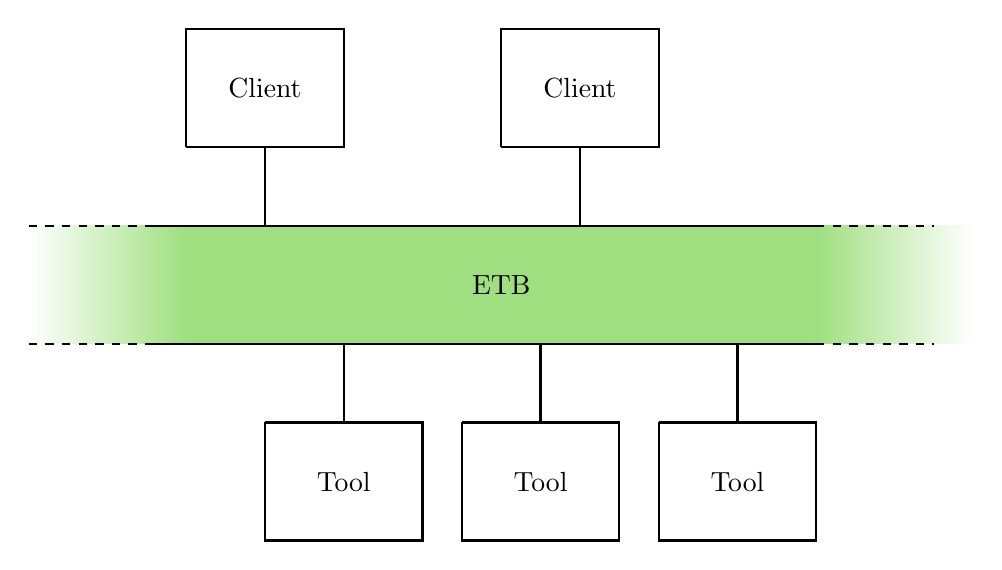
\begin{tikzpicture}
  \shade [left color=white, right color=-red!75!green!50!blue]
         (0,0) rectangle (2, 1.5);
  \shade [right color=white, left color=-red!75!green!50!blue]
         (10,0) rectangle (12, 1.5);
  \fill [color=-red!75!green!50!blue] (2,0) rectangle (10, 1.5);

  \draw[thick, dashed]
       (0,0)--(1.5,0) (10,0)--(11.5,0) (0,1.5)--(1.5,1.5) (10,1.5)--(11.5,1.5);
  \draw[thick] (1.5,0)--(10, 0) (1.5,1.5)--(10,1.5) (6,0.75) node {ETB};


  \draw[thick]
       (4,0)--(4,-1) (3,-1)--(5,-1)--(5,-2.5)--(3,-2.5)--(3,-1)
       (4,-1.75) node {Tool};
  \draw[thick]
       (6.5,0)--(6.5,-1) (5.5,-1)--(7.5,-1)--(7.5,-2.5)--(5.5,-2.5)--(5.5,-1)
       (6.5,-1.75) node {Tool};
  \draw[thick]
       (9,0)--(9,-1) (8,-1)--(10,-1)--(10,-2.5)--(8,-2.5)--(8,-1)
       (9,-1.75) node {Tool};

  \draw[thick]
       (3,1.5)--(3,2.5) (2,2.5)--(4,2.5)--(4,4)--(2,4)--(2,2.5)
       (3,3.25) node {Client};
  \draw[thick]
       (7,1.5)--(7,2.5) (6,2.5)--(8,2.5)--(8,4)--(6,4)--(6,2.5)
       (7,3.25) node {Client};

 \end{tikzpicture}
\caption{ETB Overview}\label{fig-etb}
\end{figure}

\section{Communication with the ETB}

Clients communicate with the ETB through XML-RPC and JSON over
XML-RPC. This means that a client can be written in any language that
has library support for XML-RPC and JSON. Examples of clients
distributed with the ETB are written in Python, other clients have
been written in Java or OCaml.

\subsection{ETB API}

The ETB supports a number of remote procedure calls. It supports the
{\tt system.listMethods} RPC that returns the list of available
procedures as well as the {\tt system.methodHelp} RPC to get a short
description of a given one.

These remote procedures take arguments that can be either data or file
references.

\subsection{Files and File References}

\subsubsection{The ETB File System}

The ETB has its own distributed filesystem: for a query to reference a
file, this files has to first be put on the ETB. If a query creates
new files, these have to be copied from the ETB to the local
filesystem by the client.

When a file is put on the ETB, the ETB returns a reference to the
file. This reference is used to pass the file to ETB procedures. The
reference contains both the path to the file and a hash of its
content, this is used to ensure correct versions of a file are used
when combining claims. For example, if we have an ETB that has a
service to compile a {\tt .c} file into a {\tt .o} file. A client that
want to use that service would:
\begin{enumerate}
\item Copy the {\tt .c} file to the ETB.
\item Make a query to get the {\tt .o} file created The answer to the query
contains a reference to the {\tt .o} file on the ETB.
\item The client can now copy the {\tt .o} to a location of its
  choice.
\end{enumerate}

\subsubsection{File and Directory API}

\begin{tabular}{|l|p{9cm}|}
  \hline
  {\tt put\_file({\it src}, {\it dst})} &
  Copy the file {\tt \it src} from the local file system to {\tt \it dst} on
  the ETB file system. Both {\tt \it src} and {\tt \it dst} should be absolute
  paths. Returns a file reference to the destination file on success.\\
  \hline
  {\tt get\_file({\it src}, {\it dst})} &
  Copy the file {\tt \it src} from the ETB file system to {\tt \it dst} on
  the local file system. {\tt \it src} should be a file reference to an ETB file
  and {\tt \it dst} should be an absolute path.
  Returns {\tt True} on success. \\
  \hline
\end{tabular}

\section{{\tt etbclientlib}: ETB Clients in Python}

As said before, ETB clients can be written using any programming
language that has library support for XML-RPC and JSON. The ETB comes
with a Python library, {\tt etbclientlib}, which provide high-level
construction to build ETB clients.

\subsection{The {\tt ETBClient} Class}

This is the main class exported by the library, it can be used
directly to create a client, or inherited from. It provides:
\begin{itemize}
\item a command line argument parser, parsing standard ETB options
  (e.g. host and port to contact to connect to the ETB). It can be
  extended with additional options.
\item a wrapper for methods making XML-RPC calls which catches XML-RPC
  errors. This wrapper can be used as a decorator and is useful for
  error handling.
\item high-level construction to communicate with an ETB, exchange
  files with the ETB, or make a query and wait for an answer from the
  ETB.
\end{itemize}

\subsubsection{Parsing Command-Line Arguments}

The class provides a parser inherited from {\tt
  argparse.ArgumentParser}. This parser recognizes standard ETB client
options such as {\tt --host} and {\tt --port} and can be extended as
any {\tt argparse.ArgumentParser}. For example, to add an anonymous
argument for a filename to an {\tt ETBClient} c:
\begin{pythoncode}
    c.parser().add_argument('FILE', help='filename')
\end{pythoncode}
The argument will be available as {\tt c.args().FILE}.

\subsubsection{Error Handling}

\subsubsection{Methods}

\subsection{Example: an {\tt asciidoc} Client}

\begin{pythoncode}
from etbclientlib import ETBClient
import sys

try:
    # We create an ETB client, and add a command line argument
    # for the file to be translated
    c = ETBClient('Asciidoc over the ETB')
    c.parser().add_argument('FILE', help='asciidoc file')

    # Put the file on the ETB
    input_file = c.put_file(c.args().FILE)

    # Do the query and get an answer
    answer = c.query_and_wait_answer('asciidoc("", "%s", Html)' %
                                     input_file)

    # Get the output file from the ETB
    c.get_file(answer['Html']['file'])

except Exception as e:
    print e
    sys.exit(1)

sys.exit(0)
\end{pythoncode}

\end{document}

\chapter{ETB Configuration}
\input{etb_config}

\section{}
If you installed ETB as described in \ref{install}, you should have
\texttt{etbd} and \texttt{etbsh} in your path.  In practice, the easiest
thing to do is to start from a directory with an \texttt{etb\_conf.ini}
file in it and run \texttt{etbsh} with a port, e.g.,
\begin{bashcode}
etbsh -p 12345 --etb
\end{bashcode}
The \texttt{--etb} flag indicates that the daemon should be started as a
subprocess.
The following subsections describe the ETB daemon and shell in more detail. 

\subsection{The \texttt{etbd} daemon}
The daemon the code that implements an ETB node; a workflow is defined by
interconnected ETB nodes, each with a set of rules and wrappers that
define a part of the overall workflow.

The \texttt{etbd} command starts an ETB node, which then
\begin{itemize}
\item reads a configuration file
\item loads rules and wrappers files
\item loads a file containing earlier claims and derivations
\item changes directory to the specified Git working repository
\item waits for messages from other nodes or clients
\end{itemize}
Several nodes may be running on a single computer, or across a network.
However, it is not a good idea to run two nodes at the same time that
could overwrite the same claims file.

It is important to understand that wrappers are run in the Git working
directory, so any input files need to be introduced from outside, either
from another node or from a client.  Most often \texttt{etbd} is started
in a directory that contains an \texttt{etb\_conf.ini} file, a
\texttt{wrapper} subdirectory, any number of rules files, and an
\texttt{etb\_git} subdirectory.  In this case, the defaults work except
for the \texttt{rule\_files} and \texttt{port}.
\begin{bashcode}
[etb]
port = 26532
wrappers_dir = wrappers
logic_file = logic.json.bz2
rule_files =
git_dir = etb_git
cron_period = 25
\end{bashcode}
The \texttt{etbd} also takes arguments
\begin{description}
\item[\texttt{-h}, \texttt{--help}] show a help message
\item[\texttt{-d}, \texttt{--debuglevel}] set the debug level, one of
\texttt{debug}, \texttt{info}, \texttt{warning}, \texttt{error}, or
\texttt{critical}.  Default is \texttt{info}.
\item[\texttt{--log}] a file to capture log messages; otherwise log
messages go to the terminal (i.e., stdout and stderr).
\item[\texttt{--config}, \texttt{-cf}] the config file to use
\item[\texttt{--port}, \texttt{-p}] the port to use
\end{description}
These arguments override the corresponding configuration file arguments.

\subsection{The \texttt{etbsh} shell}
The \texttt{etbsh} is a shell client that allows for interaction with an
ETB network.  It can also start up an \texttt{etbd} daemon and connect to
it, as shown above.  The \texttt{etbsh} takes arguments
\begin{description}
\item[\texttt{-h}, \texttt{--help}] show a help message
\item[\texttt{--host}] an ETB host URL, default localhost
\item[\texttt{--port}, \texttt{-p}] the port to use
\item[\texttt{--name}, \texttt{-n}] an etb name (used in proxying)
\item[\texttt{--batch}] run in batch mode, using stdin or a SCRIPT
\item[\texttt{--etb}] run \texttt{etbd}, from the specified directory if
given, else the current directory
\item[SCRIPT] is an \texttt{etbsh} load file, see below.
\end{description}

The \texttt{etbsh} shell takes a number of commands:
\begin{description}
\item[\texttt{help} [\emph{command}]]{Help for the given \emph{command},
or a summary of all commands if no \emph{command} given.}
\end{description}


\section{ETB Language}
ETB is best viewed as an extension of Datalog.  An ETB program consists of
\emph{sentences}, and the main results are \emph{claims} that are kept in
the claims table.  In order to increase the expressiveness, ETB uses a
JSON-like extension.

\subsection{Lexical}
The basic lexical tokens are identifiers, strings, and numbers.
Identifiers are any sequence of characters, except for space, \texttt{=},
colon, period, question mark, comma, quote marks (single, double, and
back), tilde (\texttt{~}, percent \texttt{\%} and various brackets
\texttt{[]()\{\}}.  Alternatively, any sequence of characters within
single quotes forms an identifier, with the usual backslash escape to
include single quotes or backslash.  Strings are any sequence of
characters within double quotes, with the backslash convention.  Numbers
are integers or floating point, with 

Identifiers are either variables or constants.  An identifier that starts
with an upper case letter is a variable, otherwise it is a constant.
Strings are enclosed in double quotes.



\bibliographystyle{plain}
\bibliography{etb}

\end{document}

%% Local Variables:
%% TeX-command-extra-options: "-shell-escape"
%% End:
